\chapter{Introduction}
\label{ch:intro}
\epigraph{To be sure, a writer cannot begin with a thesis; he must rather use his writerly sensitivity to intuit what is going on, even if he cannot understand its implications.}{\textsc{Gary Morson}, \textit{How the great truth dawned}}
%\epigraph{If you do not know where you come from, then you don't know where you are, and if you don't know where you are, then you don't know where you're going. And if you don't know where you're going, you're probably going wrong.}{Terry Pratchett}
 
%Gary Saul Morson, How the great truth dawned
%https://www.newcriterion.com/issues/2019/9/how-the-great-truth-dawned

%Taken from https://en.wikipedia.org/wiki/R.U.R.

%The Indian king Ajatashatru, who reigned in the fifth century BCE, 



In this dissertation, we present a general approach to improve visual egomotion estimation for mobile autonomous platforms. Such mobile \textit{automata} have been a part of human culture since antiquity. In ancient Greek mythology, Hephaestus--the `patron of invention and technology' \citep{MayorGodsRobots2019}--was said to have forged autonomous handmaidens that assisted him in his workshop. In ancient India, the king Ajatashatru was said to use \textit{bhuta vahana yanta} (`spirit movement machines') to protect the relics of Gautama Buddha after his death in the fourth century BCE. According to Burmese legend, the bhuta vahana yanta of Ajatashatru were made with stolen secrets from a group Greco-Roman `roboticists' named the \textit{yantakara}. The methods of the yantakara were closely guarded, and mechanical assassins were said to pursue those who attempted to disseminate them\footnote{Disseminate this document at your own risk.} \citep{MayorGodsRobots2019}.

In the millennia since, mobile automata have been largely documented only in isolated demonstrations (e.g., the programmable cart of Hero of Alexandria or the `autonomous' knight of Leonardo da Vinci) or relegated to the pages of literary work (e.g., Shelley's \textit{Frankenstein}). Although the secrets of the yantakara may never be rediscovered, the centuries-long pursuit of true autonomy has finally started to yield techniques and machinery that show great promise in aiding humanity in the twenty-first century and beyond.

\section{Egomotion Estimation}
One of said techniques is \textit{egomotion} estimation: the process of computing changes in position and orientation of a moving platform from onboard measurements.  The basic principle of egomotion estimation---the method of \textit{dead reckoning}---has been used since ancient times to determine the position of a ship at sea. Although almanacs combined with star measurements can yield \textit{latitude} estimates during the night, the problem of longitude estimation was not solved until the 18th century\footnote{With the development of the marine chronometer by John Harrison.}. As a result, marine navigators could only rely on relative ship speed measurements paired with magnetic heading to infer east-west motion. In a similar process, early aviators computed egomotion through magnetic heading, airspeed, and an estimate of prevailing winds. Although all dead-reckoning-based egomotion estimates will exhibit unbounded error growth, these early methods were particularly inaccurate and required regular corrections through known landmarks.\footnote{Perhaps the most famous example of dead-reckoning error was made by Christopher Columbus in 1492. He believed he had reached the \textit{Indies} (modern Indonesia) but had really arrived in the Bahamas.} In the twentieth century, the goals of inter-continental flight and space exploration necessitated the development of highly accurate egomotion sensors (e.g., gimballed inertial sensors like accelerometers and gyroscopes) and an associated set of estimation techniques that could compute egomotion without human intervention (e.g., the Kalman filter \citep{Grewal2010-ts}).

\begin{wrapfigure}{r}{0.5\textwidth}
	\centering
	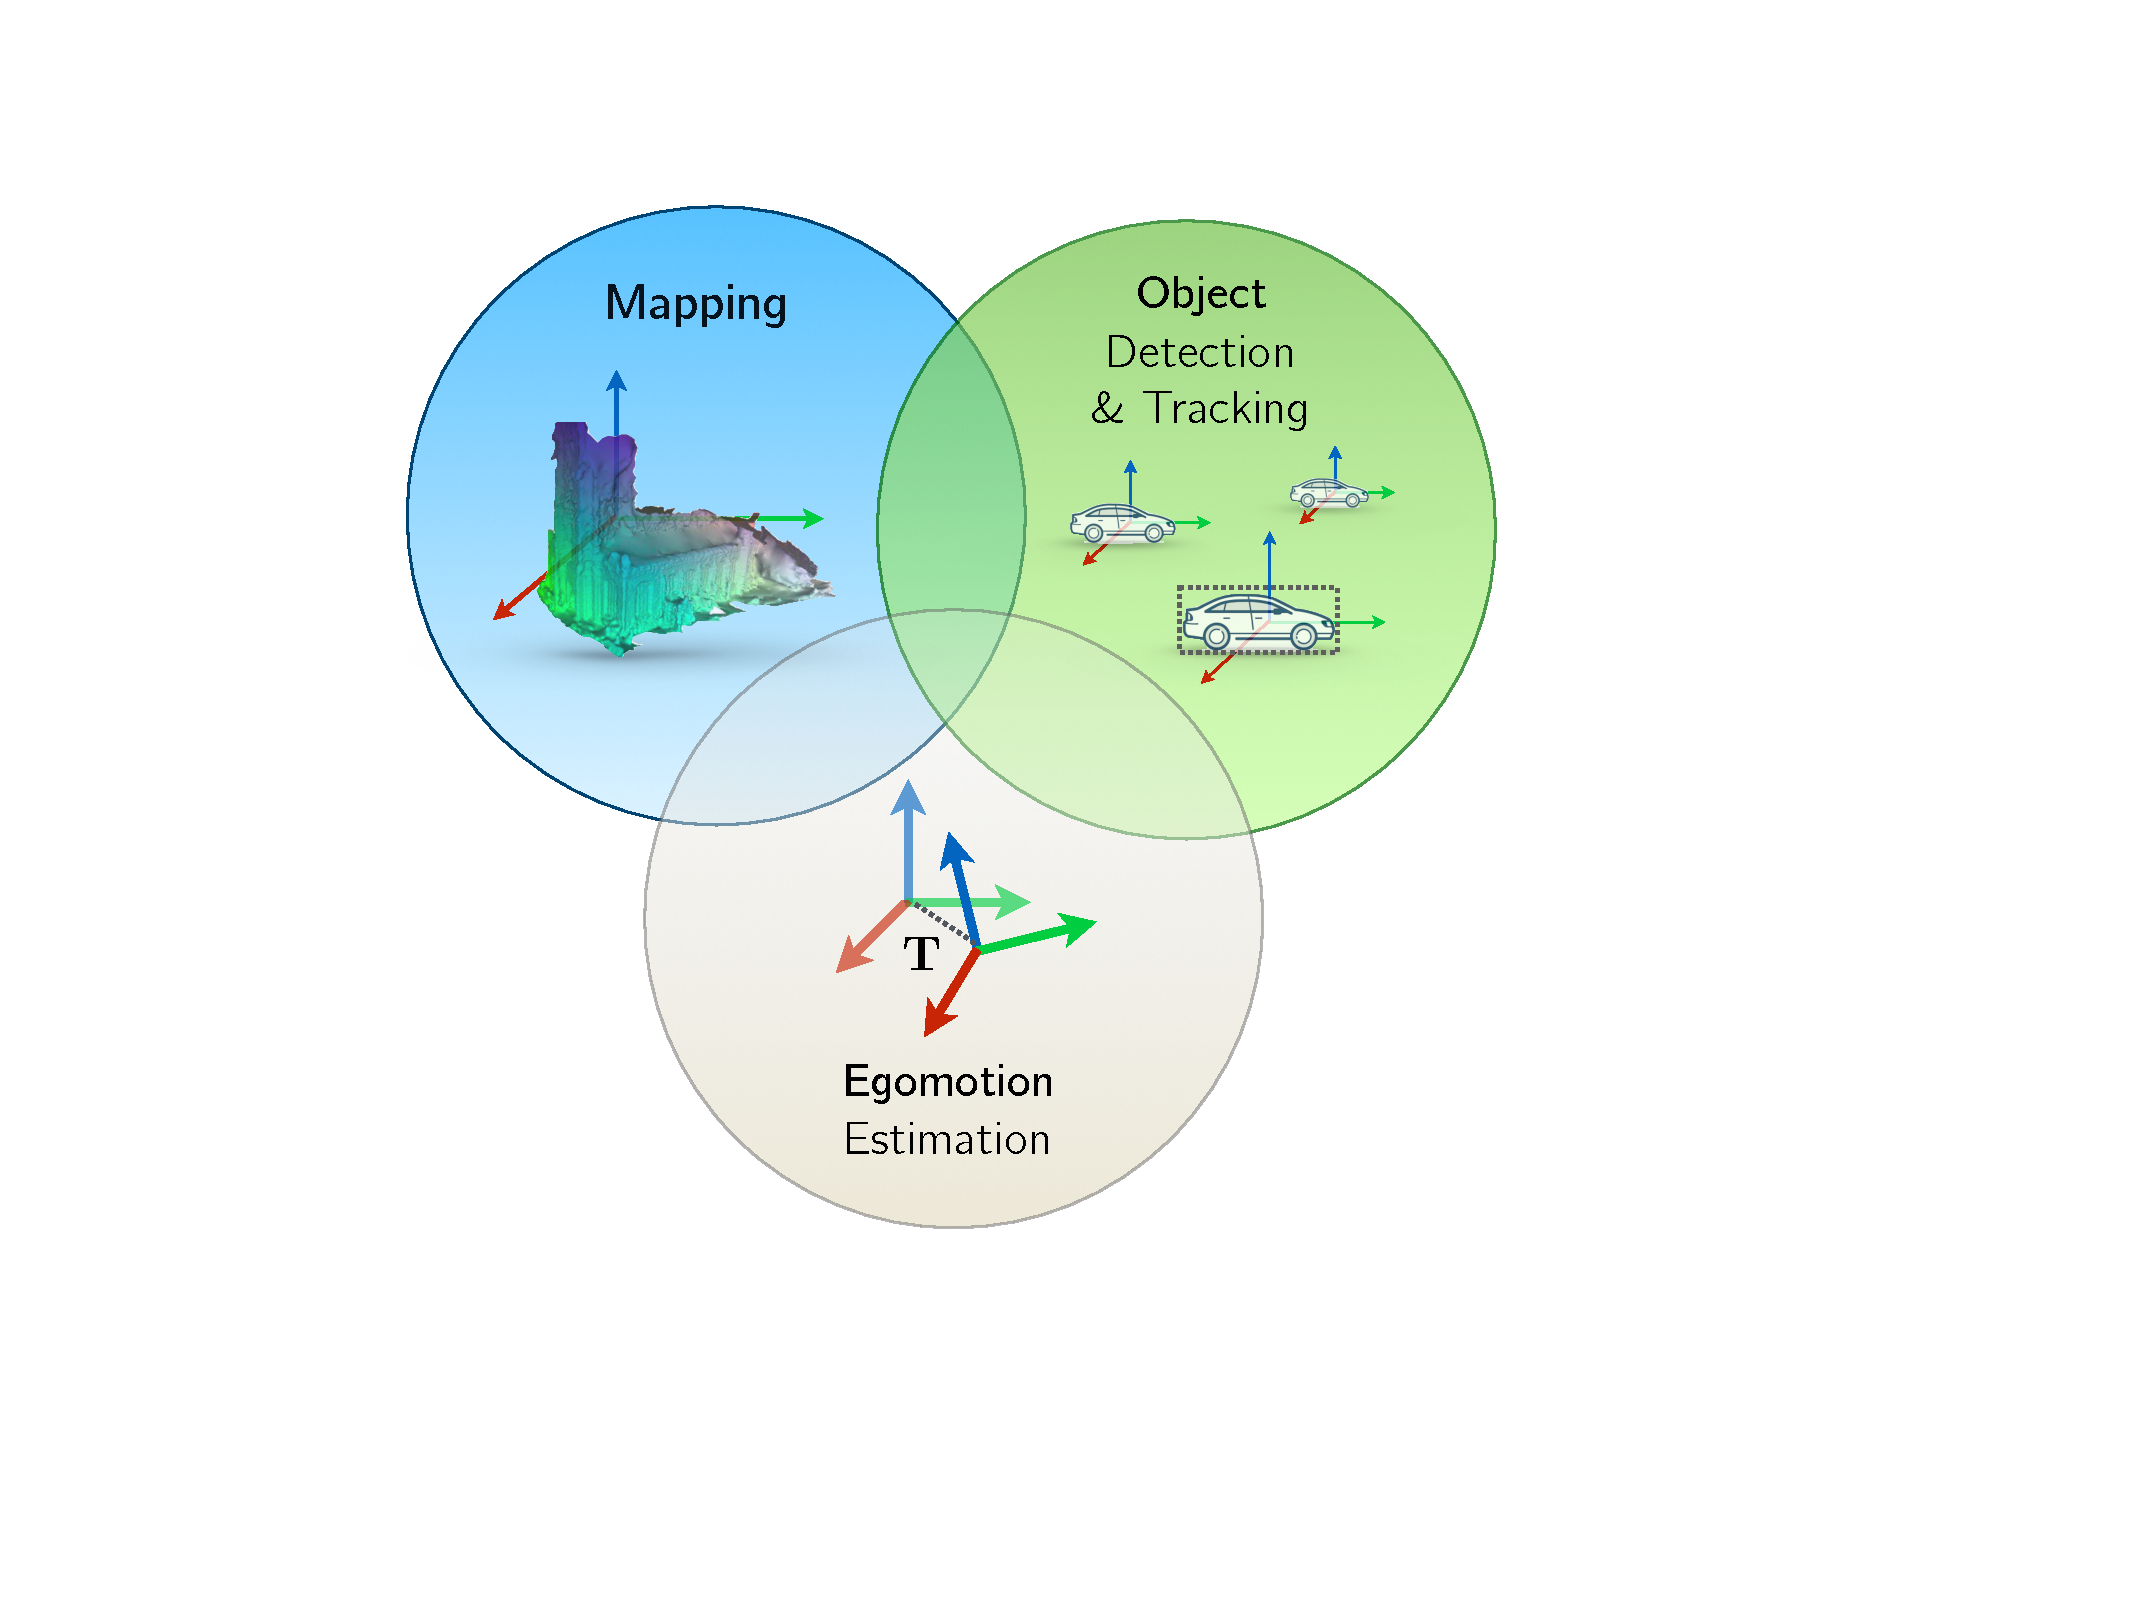
\includegraphics[width=0.48\textwidth]{introduction/venn_perception}
	\caption{Visual egomotion estimation can be used in tandem with other visual estimation techniques.}
	\label{fig:intro_state_venn}
	\vspace{-1.5em}
\end{wrapfigure}

Further, the development of extra-planetary rovers motivated the development of a new approach to egomotion estimation. Although ground vehicles can infer motion through \textit{wheel odometry} (integrating wheel rate and orientation encoder measurements into a kinematic model), this approach can be highly inaccurate on surfaces that induce wheel slip (e.g., the rock and sand covered surface of Mars). To address this, a number of researchers in the 1980s developed the technique of \textit{visual} odometry \citep{Scaramuzza2011-qr} (or VO), as a way to compute egomotion using images collected sequentially. VO is closely related to the techniques of \textit{bundle adjustment} \citep{triggs_bundle_2000} and \textit{structure from motion} that were initially developed to automate the reconstruction of cold-war-era reconnaissance imagery.






% Modern mobile autonomy was largely born out of  .
% 
%https://mars.nasa.gov/resources/22342/opportunity-legacy-pan-true-color/
\begin{figure}
  \begin{center}
  	\vspace{-10pt}
    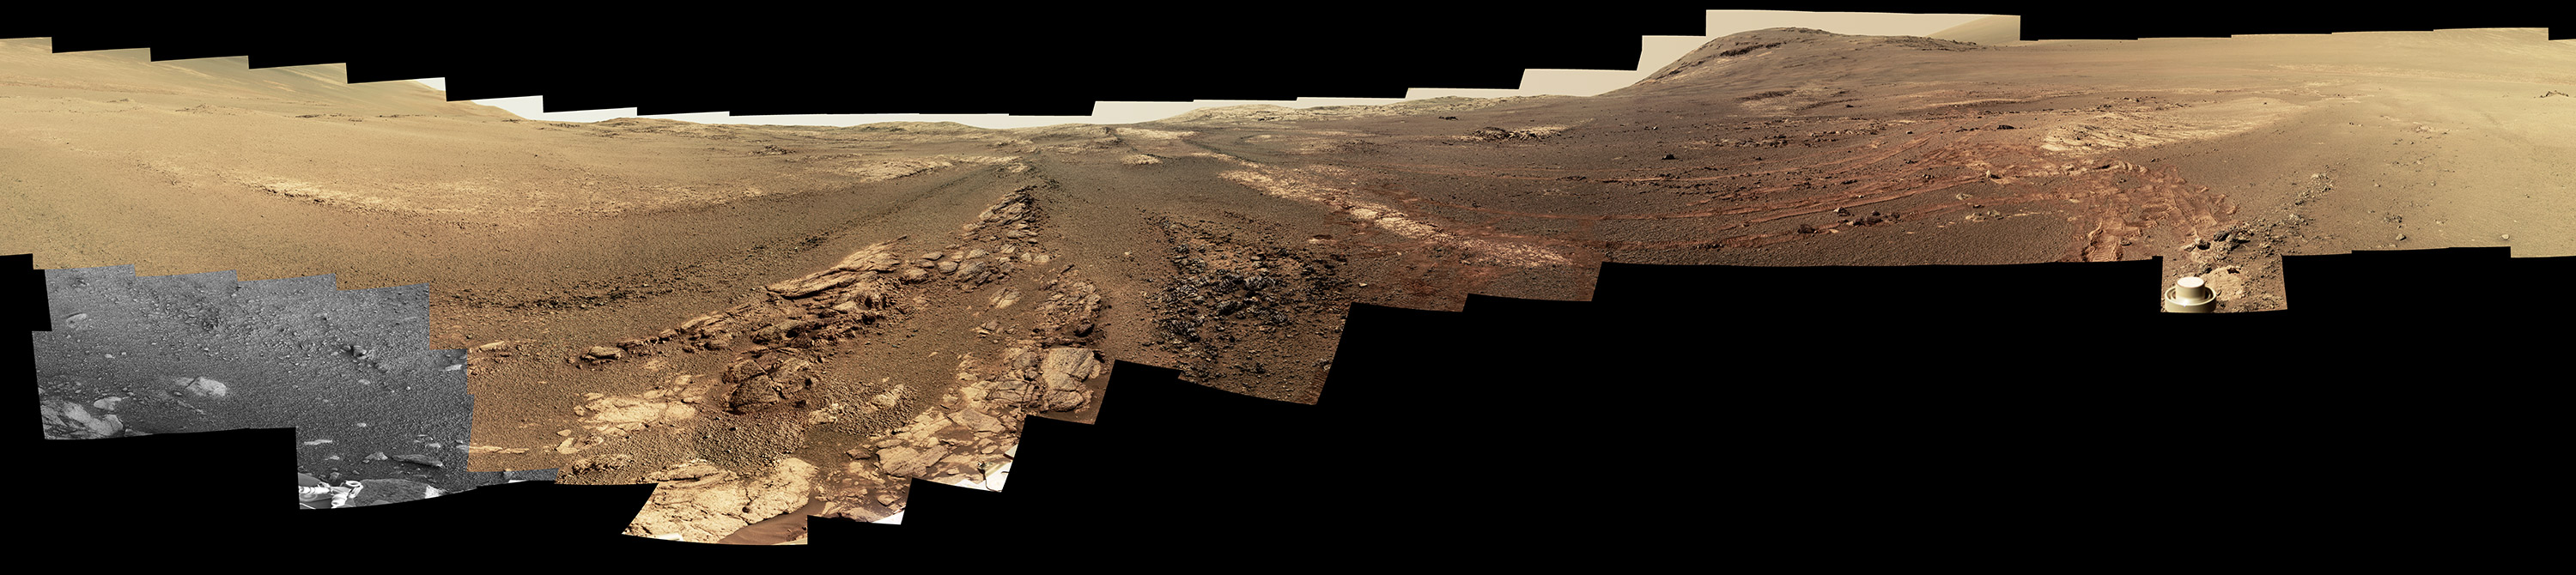
\includegraphics[width=0.95\textwidth]{introduction/pancam-panorama-opportunity}
     \vspace{-15pt}
  \end{center}
  \caption{The last 360 degree panorama taken by the PanCam apparatus of the Mars Exploration Rover, \textit{Opportunity}, at its final resting place on Mars, the western rim of the Endeavour Crater. Contact with \textit{Opportunity} was lost shortly after this was captured, due to a severe dust storm (credit: NASA/JPL-Caltech/Cornell/ASU).}
  \vspace{-5pt}
  \label{fig:into_rur}
\end{figure}





%\begin{figure}
%         \centering
%\def\firstcircle{(0,0) circle (2cm)}
%\def\secondcircle{(60:2.75cm) circle (2cm)}
%\def\thirdcircle{(0:2.75cm) circle (2cm)}
%\scalebox{0.75}{
%\begin{tikzpicture}
%    \begin{scope}[shift={(3cm,-5cm)}, fill]
%        \fill[green!80,opacity=0.5] \firstcircle;
%        \fill[blue,opacity=0.5] \secondcircle;
%        \fill[black,opacity=0.5] \thirdcircle;
%        \draw \firstcircle node [yshift=-1ex,xshift=-2.5ex,align=center] {C. Mapping};
%        \draw \secondcircle node [above,color=white,align=center] {A. Egomotion\\estimation};
%        \draw \thirdcircle node [yshift=-1ex,xshift=3ex,color=white,align=center] {B. Object\\tracking};
%        \draw[->] (1.2,0.8) -- (3.7,3) node[right,align=left] {State\\Estimation};
%    \end{scope}
%\end{tikzpicture}         
%}
%        \caption{Venn diagrams of modern mobile autonomy.}
%        \label{fig:intro_three_venn}
%\end{figure}


 %Add some discussion about computer science vs. robotics research
 
In the last decade, the development of compact, relatively-inexpensive, high resolution cameras has made vision-based estimation ubiquitous in mobile autonomous applications. In addition to computing egomotion, camera data can be used to build detailed maps of an environment (which can often be solved in tandem with egomotion estimation, resulting in a technique named simultaneous localization and mapping, or SLAM \citep{Cadena2016-ds}), as well as detect, track and avoid other objects (see \Cref{fig:intro_state_venn}). 

\section{A Visual \textit{Pipeline}}

\begin{figure}
\begin{center}
		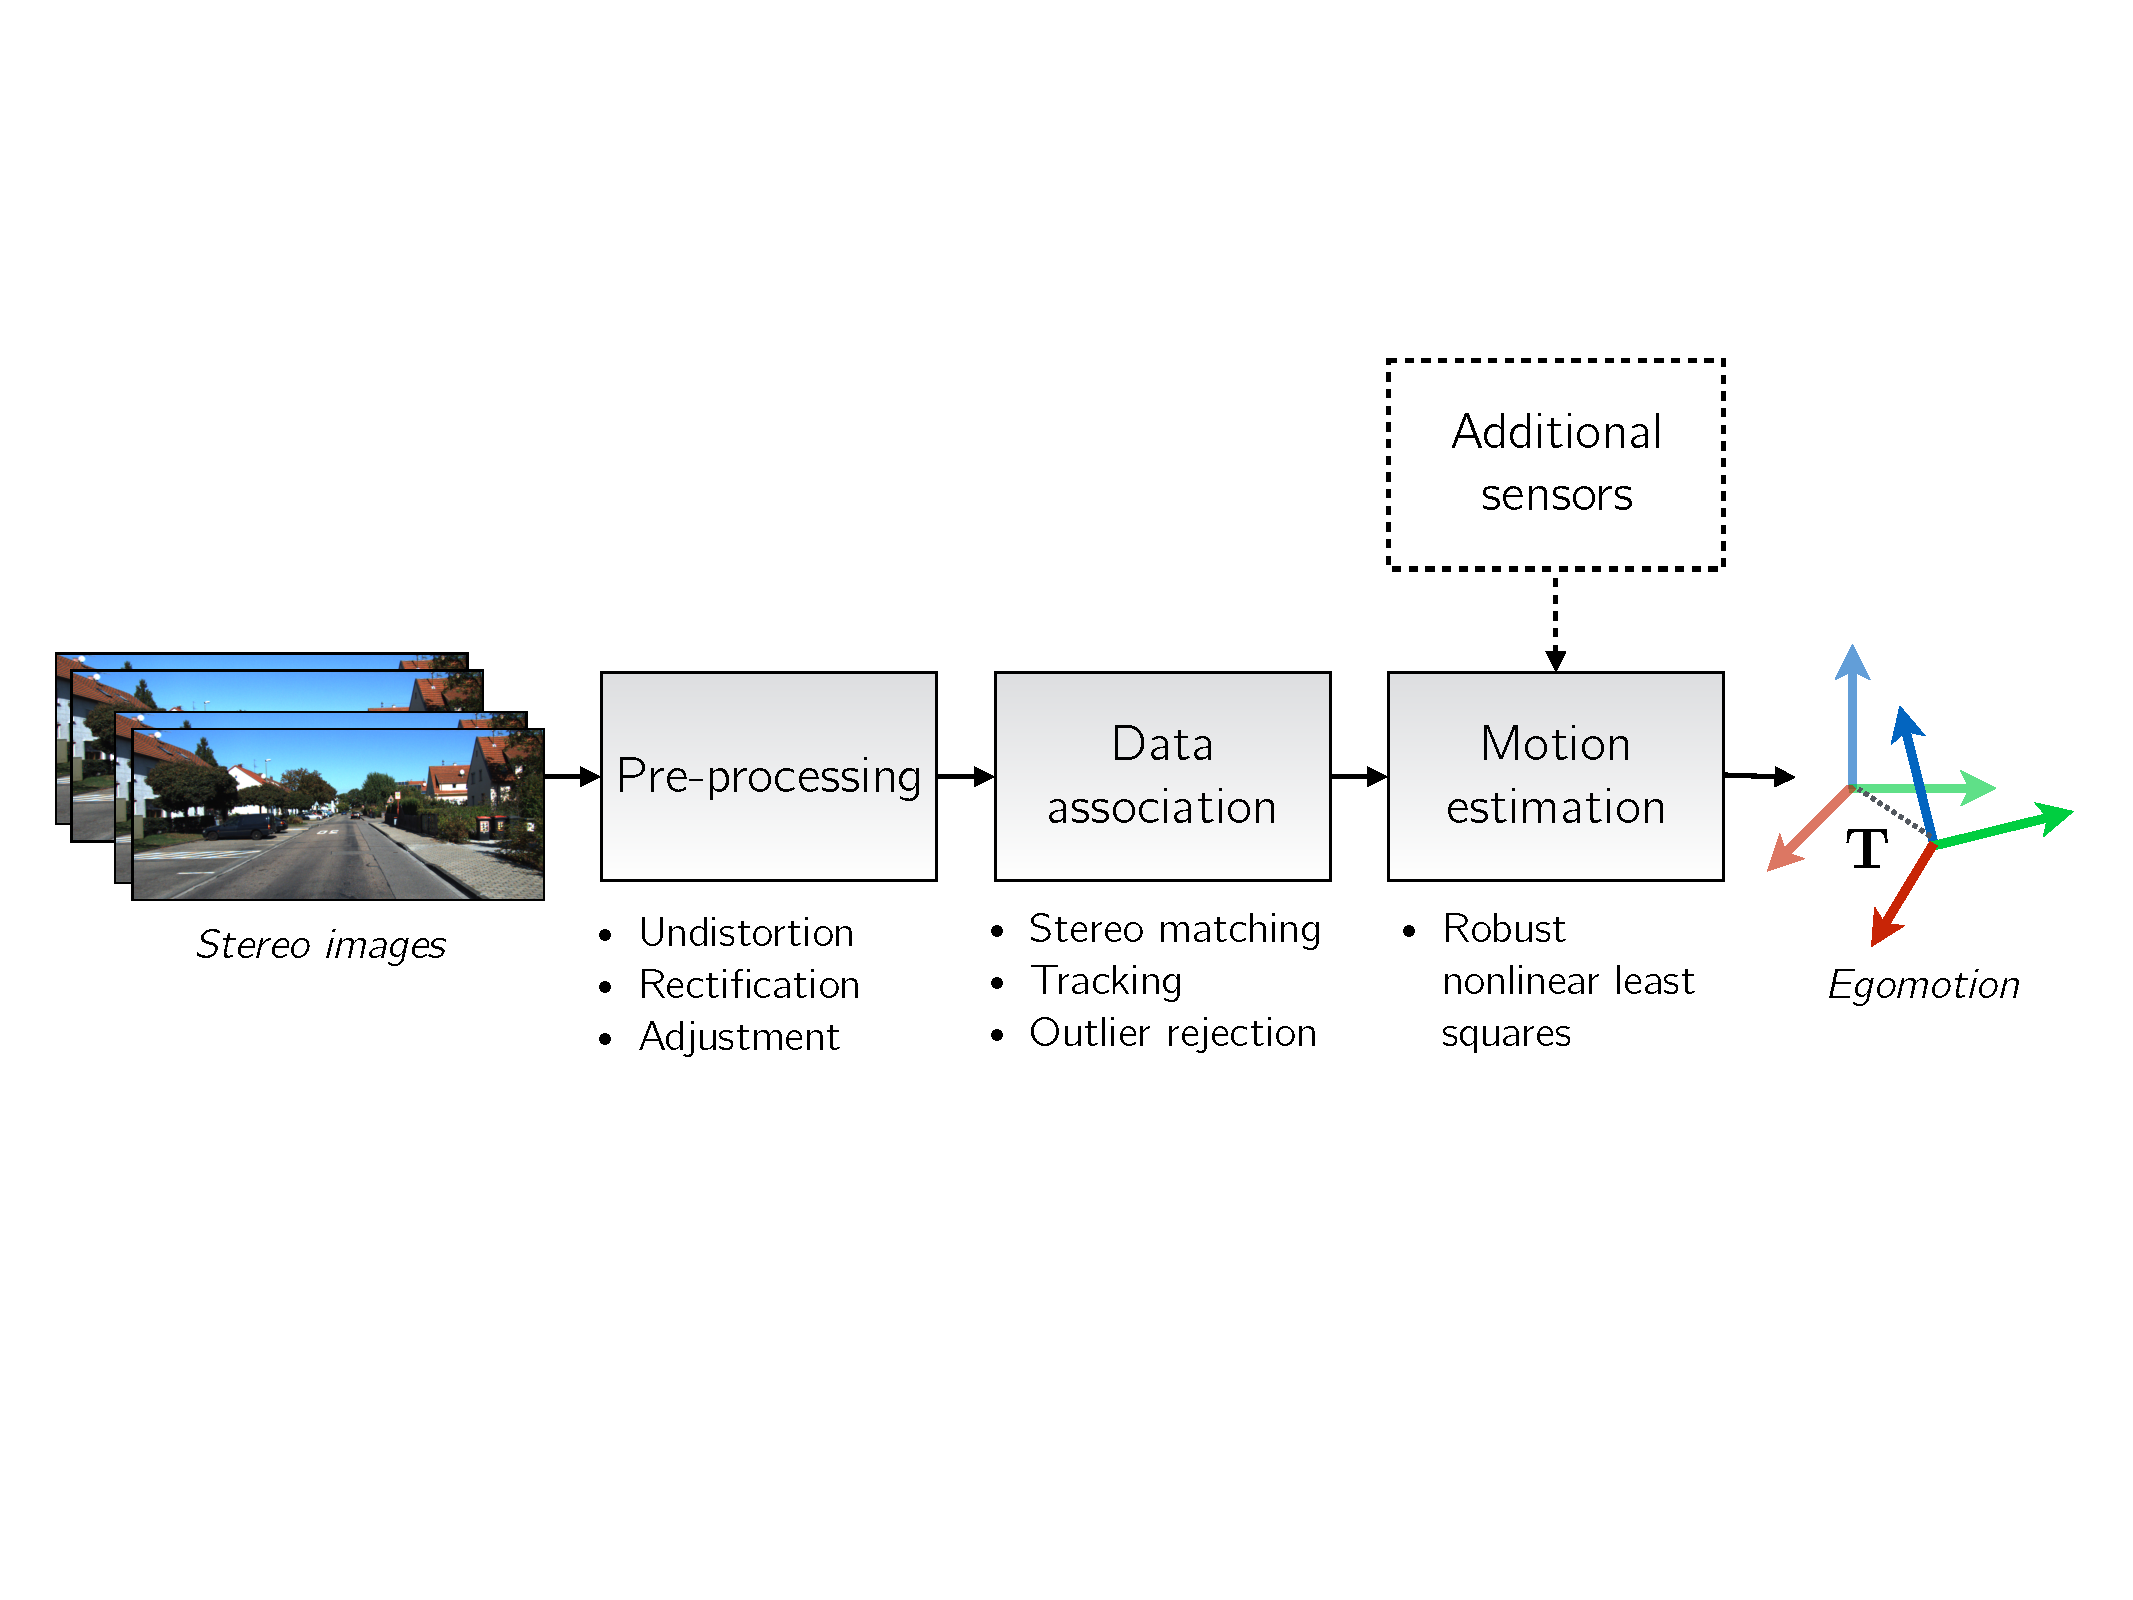
\includegraphics[width=0.98\textwidth]{introduction/vo_pipeline.pdf}
		\caption{A `classical' visual odometry pipeline consists of several distinct components that have interpretable inputs and outputs.}
  	\label{fig:intro_vo_pipeline}
\end{center}
\end{figure}


Central to \textit{classical} visual odometry algorithms (which, in this context, refers to the bulk of VO research published during what \cite{Cadena2016-ds} call the \textit{classical} and \textit{algorithmic-analysis} ages of VO and SLAM research between 1986 and 2015) is the idea of a pipeline. A pipeline consists several distinguishable blocks that have interpretable inputs and outputs.  By carefully processing information contained within sensor data, pipelines facilitate the construction of complex state estimation architectures that can fuse observations from sensors of varied modality to create rich models of the external world and infer the state of a mobile platform within it. In this dissertation, we will largely deal with the improvement of a baseline VO pipeline-- we illustrate its major components in \Cref{fig:intro_vo_pipeline}. 

Such Classical VO pipelines (e.g., \cite{Leutenegger2015-fk, Cvisic2015-mt, Tsotsos2015}) have achieved impressive localization accuracy on trajectories spanning several kilometres by carefully extracting and tracking sparse visual features (using \textit{hand-crafted} algorithms) across consecutive images. Simultaneously, significant effort has gone to developing localization pipelines that eschew sparse features in favour of \textit{dense} visual data \citep{Alcantarilla2016-kv, forster2014svo}, typically relying on loss functions that use direct pixel intensities. 

In the last five years, a significant part of the visual state estimation literature has also focused on the idea of replacing classical pipelines with parametric modelling through deep convolutional neural networks (CNNs) and data-driven learning. Although initially developed for image classification  \citep{LeCun2015-qf}, CNN-based measurement models have been applied to numerous problems in geometric state estimation (e.g., homography estimation \citep{DeTone2016-ue}, single image depth reconstruction \citep{Garg2016-ip},  camera re-localization \citep{Kendall2016-zf}, place recognition \citep{Sunderhauf2015-is}). A number of recent CNN-based approaches have also tackled the problem of egomotion estimation, often purporting to obviate the need for classical visual localization pipelines by learning pose changes \textit{end-to-end}, directly from image data (e.g., \cite{Melekhov2017-dl}, \cite{Handa2016-hm}, \cite{Oliveira2017-lt}).

Despite this surge of excitement, significant debate has emerged within the robotics and computer vision communities regarding the extent to which deep models should replace existing geometric state estimation algorithms. Owing to their representational power, deep models may move the onerous task of selecting `good' (i.e., robust to environmental vagaries and sensor motion) visual features from the roboticist to the learned model. By design, deep models also provide a straight-forward formulation for using \textit{dense} data while being flexible in their loss function, and taking full advantage of modern computing architecture to minimize run-time. Despite these potential benefits, end-to-end regression techniques for state estimation often generalize poorly to new environments, come with few analytical guarantees, and provide only point estimates of latent parameters (see \Cref{tab:intro_classical_vs_deep} for more details). Indeed, the most accurate visual egomotion pipelines at the time of writing\footnote{Based on the KITTI Odometry benchmark leaderboard at \url{http://www.cvlibs.net/datasets/kitti/eval_odometry.php}.} remain largely those based on carefully selected sparse features. Furthermore, there is recent empirical evidence \citep{Zhou2019-se} that suggests that designing a pipeline with interpretable components (e.g., optical flow, scene segmentation) is crucial to generalization on various visual tasks. 

\begin{figure}
\begin{center}
		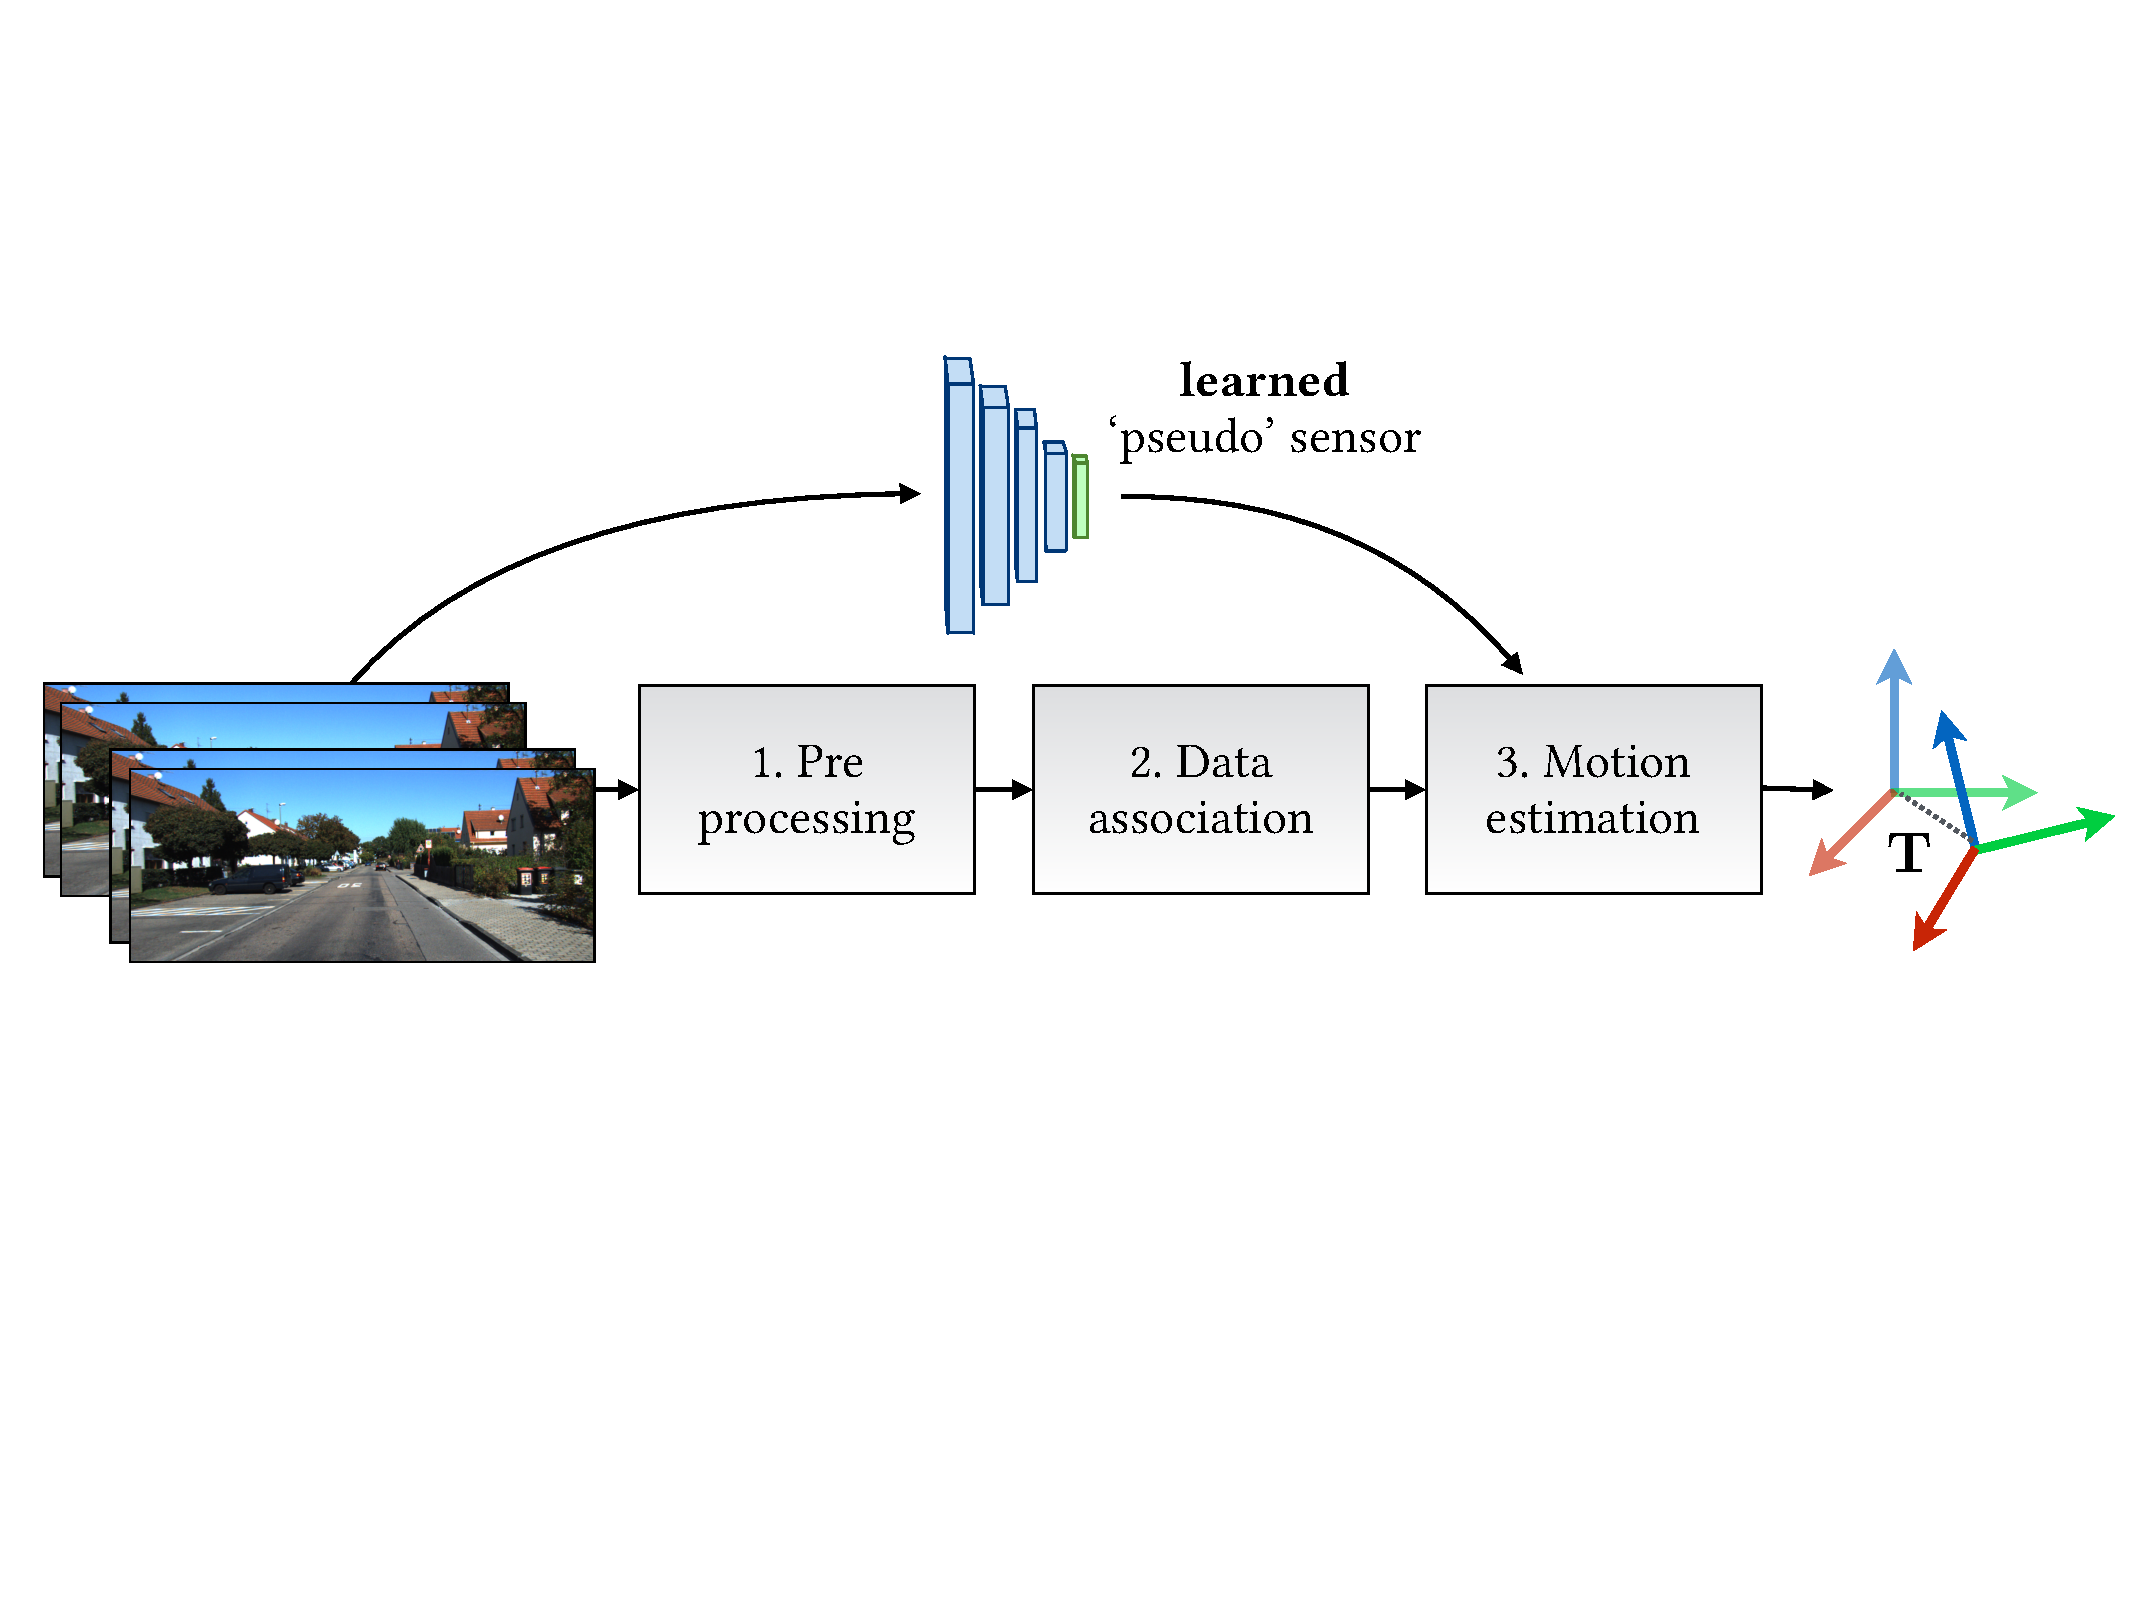
\includegraphics[width=0.98\textwidth]{introduction/pseudo_sensor.pdf}
		\caption{A learned \textit{pseudo-sensor} extracts latent information from the same data stream.}
  	\label{fig:intro_pseudo_sensor}
\end{center}
\end{figure}


\begin{table}[h!]
	\caption{A comaprison of pipelines and end-to-end deep models for visual egomotion estimation.}
	\begin{threeparttable}
	\begin{tabular}{m{0.18\textwidth}m{0.38\textwidth}m{0.38\textwidth}}
		\toprule
		& \textbf{Classical Pipelines} & \textbf{Deep Models} \\ \midrule  
		\textit{Maturity} & Decades of literature \& domain knowledge & Nascent with few uses in mobile autonomy \\
		& & \\
		\textit{Interpretability} & Good, each component has interpretable input and output & Poor, often with no interpretable intermediate outputs \\
		& & \\
		\textit{Uncertainty} & Foundational to \textit{probabilistic robotics} & Few nascent methods (Monte-carlo Dropout \citep{Gal2016-ny}, Bootstrap \citep{Osband2016})  \\
		& & \\
		\textit{Robustness} & Empirically generalizable \citep{Zhou2019-se} & Highly dependant on training data\\
		& & \\
		\textit{Flexibility} & Limited by ingenuity of designer & Limited by training data \\
		\bottomrule
	\end{tabular}
\end{threeparttable}
\label{tab:intro_classical_vs_deep}
\end{table}

\section{The Learned Pseudo-Sensor}

As state estimation enters the robust-perception age \citep{Cadena2016-ds}, algorithms that work in limited contexts will need to be adapted and augmented to ensure they can operate over longer time-periods, and through sundry environments. Towards this end, we introduce the paradigm of the \textit{learned pseudo-sensor}. Learned pseudo-sensors allow one to retain the benefits of classical state estimation pipelines while leveraging the representational power of modern data-driven learning techniques. Instead of completely replacing the classical pipeline, herein we present four ways in which machine learning can be used to train a hyper-parametric model that extracts latent information from an existing visual and inertial data stream. By fusing the output of these sensors with the output of the pipeline, we can make the final egomotion estimates more accurate and more robust to difficult-to-model effects (\Cref{fig:intro_pseudo_sensor}). To accomplish this fusion, we rely on two approaches. The first, which we call Predictive Robust Estimation (PROBE, \Cref{ch:probe}), uses the paradigm of a pseudo-sensor to build a heteroscedastic noise model from extant visual-inertial data. By predicting uncertainty information, PROBE effectively re-scales a robust loss function to better account for deleterious visual effects. The second approach (used by Sun-BCNN, DPC-Net, and HydraNet,  \Cref{ch:sun-bcnn,ch:dpc,ch:hydranet} respectively) produces geometric quantities (probabilistic estimates of an illumination source, $\LieGroupSE{3}$ corrections to existing egomotion estimates, and independent probabilistic rotation estimates, respectively), that can be fused with the original pipeline through a factor graph optimization routine.

%\section{Outstanding Issues in the Field}

%\subsection{The limits of homoscedastic noise models}
%
%Although several state-of-the-art state estimation pipelines  \citep{Leutenegger2015-fk, Cvisic2015-mt} leave observation uncertainty associated with sensor measurements as a static tuning parameter, recent work \citep{Vega-Brown2014-sb, Hu2015-uw} suggests that using a stationary, homoscedastic noise in observation models can often reduce the consistency and accuracy of state estimates. This is especially true for complex, inferred measurement models. In foot-mounted navigation, the inferred zero velocity detector may be more or less informative depending on the exact type of motion and individual gait. In visual data, inferred visual observations can be degraded not only due to sensor imperfections (e.g. poor intrinsic calibration, digitization effects, motion blur), but also as a result of the observed environment (e.g. self-similar scenes, specular surfaces, textureless environments). Indeed, robust costs \cite{Alcantarilla2016-kv, MacTavish2015-wt, Agarwal2013-jq} and whiteness tests \citep{Tsotsos2015} have commonly been used to alleviate the problem of poor noise modelling, but more work is required to better learn uncertainty in complex measurement models.
%
%
%\subsection{Deep, learned models with no uncertainty estimates}
%
%Although the paradigm of deep neural networks has resulted in several significant achievements in the fields of computer vision \citep{LeCun2015-qf}, these types of models have largely focused on point estimates (in either regression or classification) without any principled uncertainty estimates. Recently, the regularization techniques of dropout and dropconnect in Convolutional Neural Networks have been linked with approximate variational inference in homoscedastic Gaussian Processes \citep{Gal2015-bf, Kendall2016-zf, McClure2016-ai}, and the statistical technique of \textit{bootstrapping} has been applied to Deep Q Networks \citep{Osband2016-jg} to infer uncertainty, but both techniques are in their infancy. Recent work \citep{Osband_undated-wl} has also suggested that the former technique of dropout-based `uncertainty' is actually a measure of \textit{risk} (i.e., stochasticity in the measurements) and not \textit{uncertainty} over state parameters. Further, the same work showed that even this risk quantification can be arbitrarily bad given a fixed dropout parameter (which is typically the case).
%
%\subsection{Integration of deep models into state estimation pipelines}
%
% To integrate the power of deep networks into state estimation algorithms, the recent literature differs in how to proceed. While some attempt to parametrize geometric transformations in their unconstrained state, and then learn the resulting state within a deep network regression optimization \citep{Costante2016-hb, Kendall2015-kh}, others integrate deep networks within outer estimation loops \citep{Haarnoja2016-ph}. Yet other work has used the neural network as an error correcting mechanism on top on an existing kinematic or dynamic model \citep{Punjani2015-pj}. This integration is made more difficult by the lack of uncertainty estimates associated with many learned measurement models in the computer vision and machine learning literature.
% 
 
\section{Original Contributions}

\begin{figure}[h!]
\begin{center}
		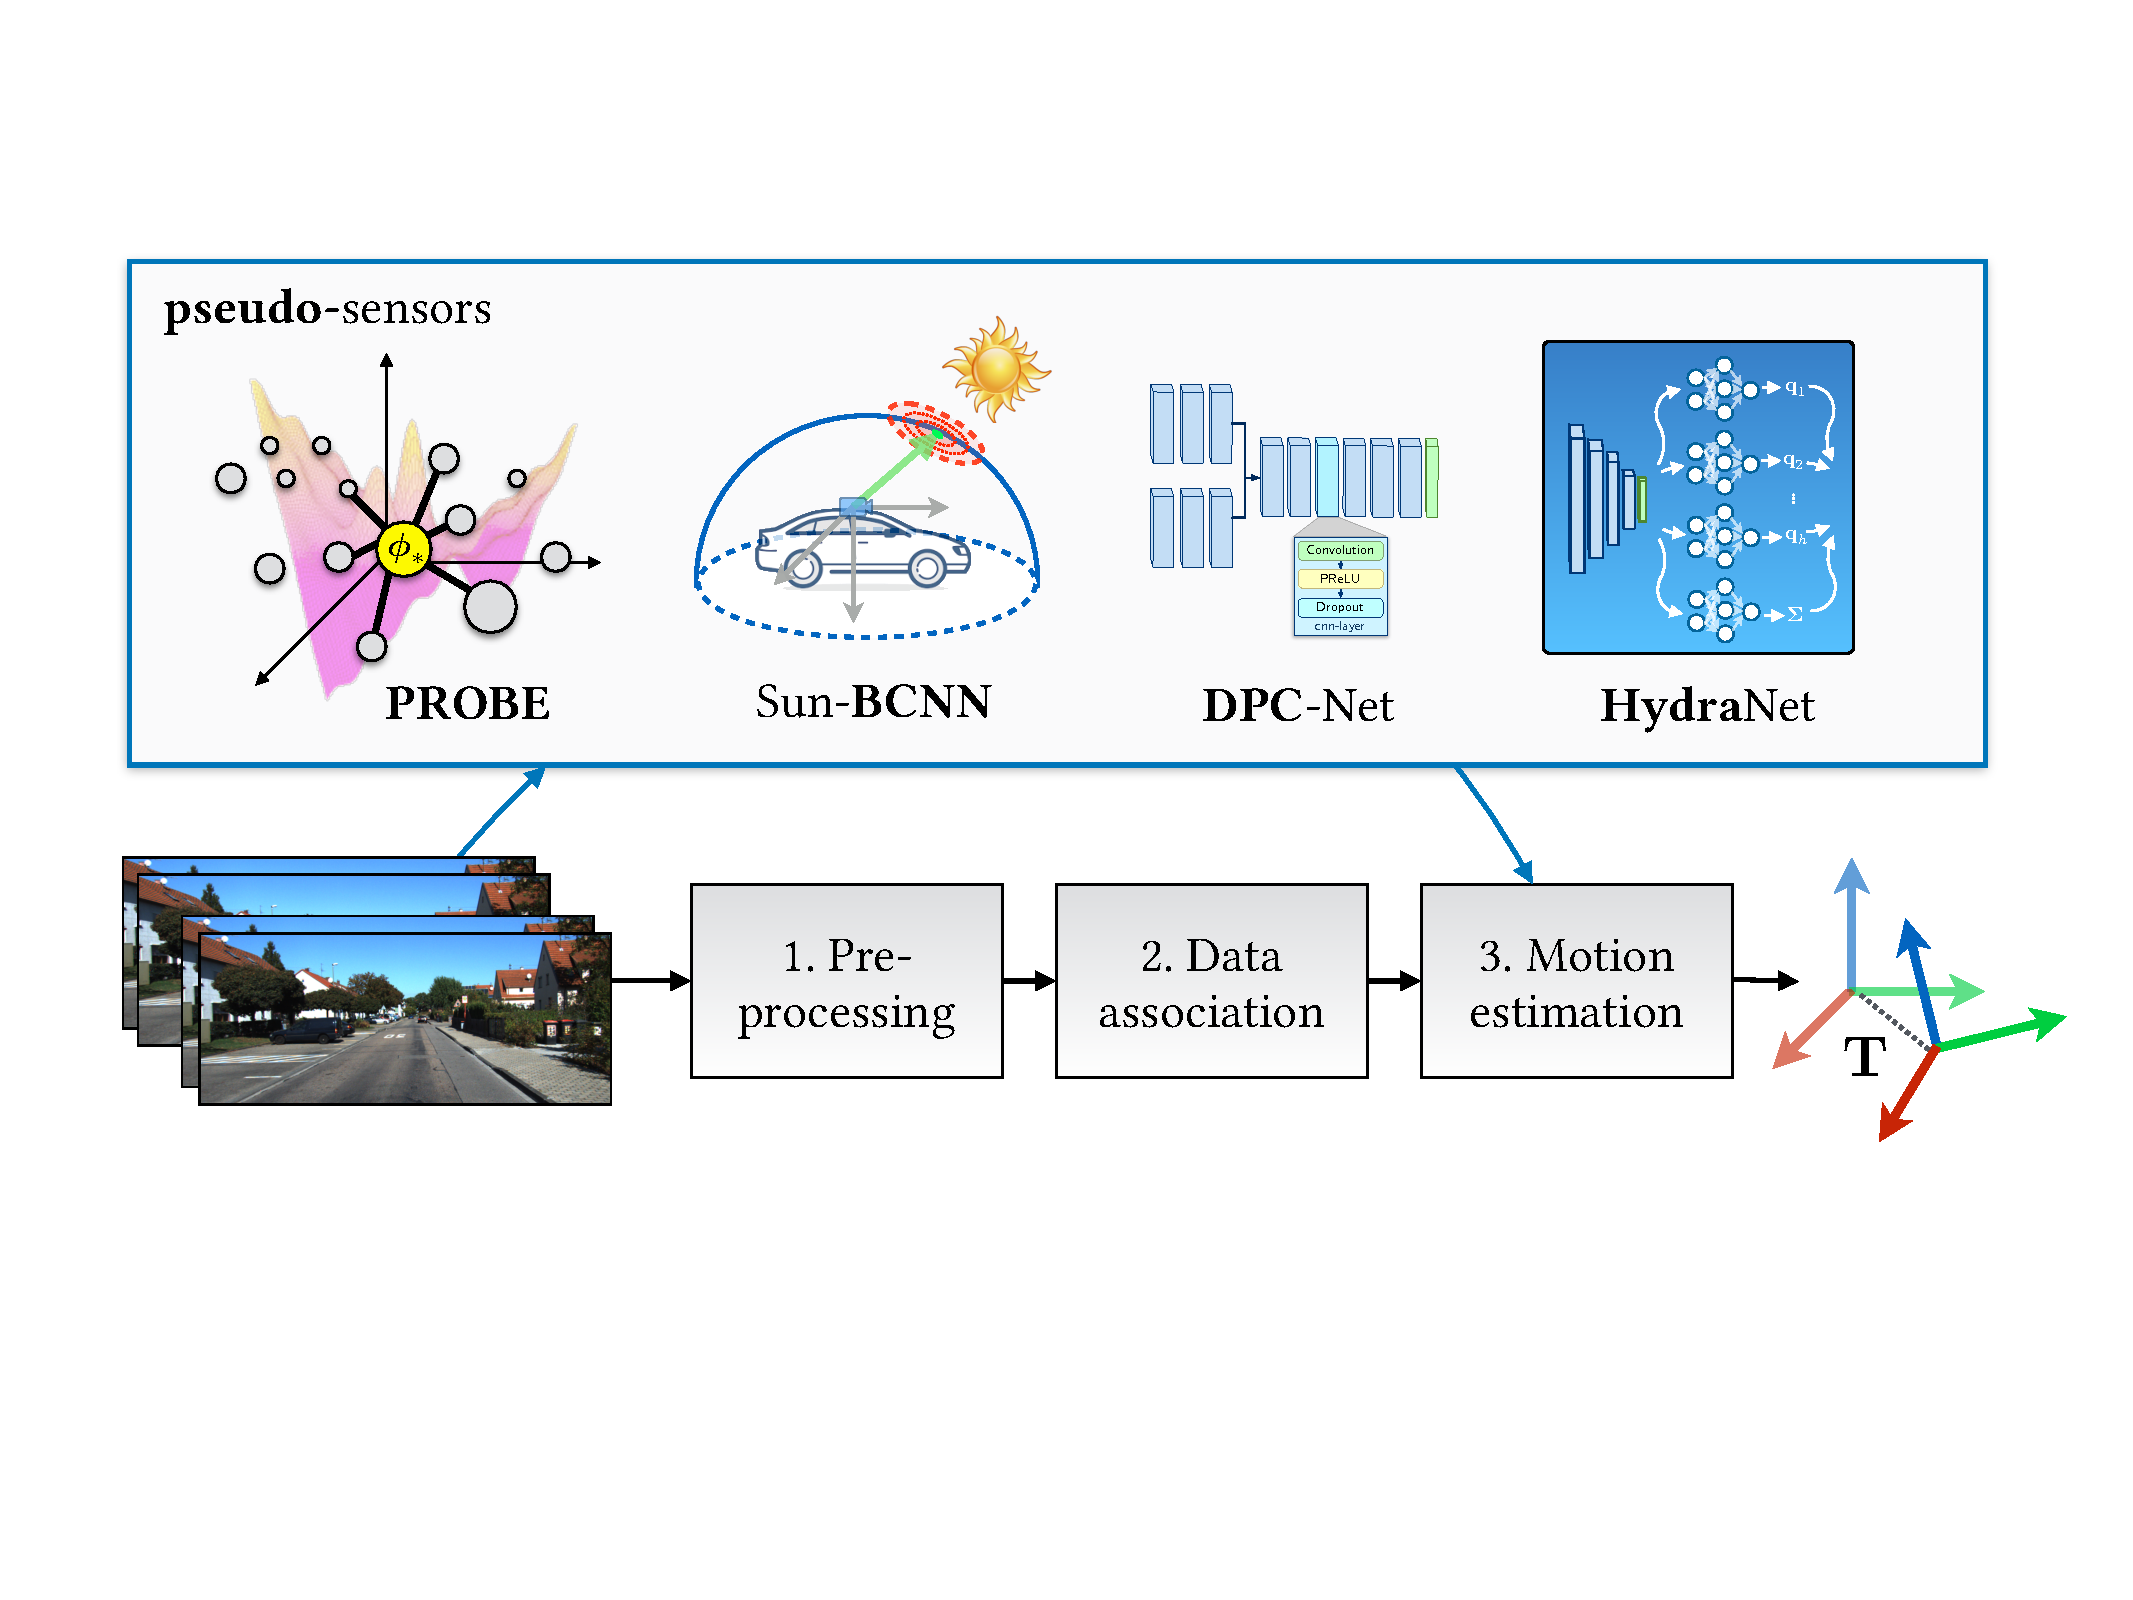
\includegraphics[width=0.98\textwidth]{introduction/all_pseudo_sensors.pdf}
		\caption{This dissertation details four examples of \textit{pseudo-sensors} that improve 'classical` egomotion estimation through data-driven learning.}
  	\label{fig:intro_pseudo_sensors}
\end{center}
\end{figure}


This dissertation consists of several published contributions under the umbrella of \textit{learned pseudo-sensors} that improve a canonical visual egomotion pipeline. Before detailing each pseudo-sensor, we present some mathematical foundations (\Cref{ch:math}) and a common baseline for an indirect stereo visual odometry pipeline (\Cref{ch:vo}) which all four methods build upon. In total, there are two journal papers and five conference papers associated with our work. Below, we briefly summarize each of the pseudo-sensors and list the publications that are associated with each.
\begin{enumerate}
\item \textbf{Predictive Robust Estimation (PROBE)},  \\
Predictive Robust Estimation (\Cref{ch:probe}, Appendix \ref{app:appendix_probe_knn}) uses the method of Generalized Kernel (GK) estimation \citep{Vega-Brown2014-sb} to derive an efficient Bayesian model for stereo tracking uncertainty based a set of training reprojection errors. By setting a prior on covariance, we derive a robust loss that can be predictively scaled to improve the accuracy and consistency of an indirect stereo visual odometry pipeline. PROBE is associated with three publications listed below. The first two publications (and Appendix \ref{app:appendix_probe_knn}) explore useful predictors for uncertainty and build a non-Bayesian isotropic covariance model. The latter publication presents the Bayesian GK approach.
\begin{itemize}
\item \bibentry{2015_Peretroukhin_PROBE},
\item \bibentry{2015_Peretroukhin_Get},
\item \bibentry{Peretroukhin2016-om}.
\end{itemize}

\item \textbf{Sun-BCNN: Learned sun sensor} \\ 
Sun-BCNN (\Cref{ch:sun-bcnn}) is a technique to infer a probabilistic estimate of the direction of the sun from a single RGB image using a Bayesian Convolutional Neural Network (BCNN). The method works much like hardware sun sensors \citep{Lambert2012-sn}, but does not requires any additional sensing equipment, and can provide mean and covariance estimates that can be readily incorporated into existing visual odometry frameworks.  It is associated with three publications listed below. Initial exploratory work was published at ISER, and the BCNN improvement was presented at ICRA. An additional journal paper summarizing the work of the prior two papers, adding data from the Canadian High Arctic and Oxford, and investigating the effect of cloud cover and transfer learning was published in the International Journal of Robotics Research, Special Issue on Experimental Robotics. 
\begin{itemize}
\item \bibentry{2017_Clement_Improving},
\item \bibentry{2017_Peretroukhin_Reducing},
\item \bibentry{2018_Peretroukhin_Inferring}.
\end{itemize}

\item \textbf{DPC-Net: Learned pose corrections} \\
Deep Pose Correction (\Cref{ch:dpc}) is an approach to improving egomotion estimates through $\LieGroupSE{3}$ pose corrections learned through deep regression with a supervised loss based on Lie theory. The Deep Pose Correction Network (DPC-Net) learns low-rate, `small' \textit{corrections} from training data that are then fused with the original estimates from the canonical pipeline. DPC-Net does not require any modification to an existing pipeline, and can learn to correct multi-faceted errors from estimator bias, sensor mis-calibration or environmental effects. It is associated with one journal publication listed below.
\begin{itemize}
\item \bibentry{2018_Peretroukhin_Deep}.
\end{itemize}

\item \textbf{HydraNet: Learned probabilistic rotation estimation}

Finally, HydraNet (\Cref{ch:hydranet}) is a multi-headed network structure that can regress probabilistic estimates of rotation (elements of the matrix Lie group, $\LieGroupSO{3}$) that account for both aleatoric and epistemic uncertainty. HydraNet builds upon results from both Sun-BCNN and DPC that show that correcting rotation is critical to accurate egomotion estimation.  Towards this end, HydraNet is designed to produce well-calibrated notions of uncertainty over $\LieGroupSO{3}$  that facilitate fusion with classical egomotion pipelines through a probabilistic factor graph formulation. It is associated with one publication:

\begin{itemize}
\item \bibentry{2019_Peretroukhin_Deep}.
\end{itemize}


\end{enumerate}

%\subsection{Software Contributions}
%
%\begin{itemize}
%\item DPC-Net
%\item SO(3) Learning
%\item \texttt{liegroups}
%\item pyslam 	
%\end{itemize}






